%!TEX root = main_arduino_intro.tex

\chapter{Temperature sensor}

Temperature is generally measured with a thermocouple. In these devices, two metals are brought together that, due to the \href{https://en.wikipedia.org/wiki/Thermoelectric_effect}{Seebeck effect}, create a temperature-dependent voltage between them. The voltages produced generally are very low and therefore require amplification before they can be read in by an \ac{adc}. Such an amplifier for a K-type thermocouple can, e.g., be found \href{https://www.adafruit.com/product/1778}{here}. In this specific case, the amplification circuit would allow us to read temperatures from -250\celsius\ to +750\celsius, i.e., a total range of 1000\celsius.

\qbox{The Arduino Micro that we are using contains eight 10\,bit \acp{adc}. Why is it very difficult to get a precise reading of the thermocouple described above using such an \ac{adc}? What would you need to implement / improve the precision?}


\section{Thermistor}

While regular thermocouples have a very wide range, this range is not required for our setup. Here we are therefore using a thermistor, which is simply a resistor that is highly temperature dependent. 

\subsection{Voltage divider}

In order to understand how we can determine the value of a thermistor with an Arduino, we first need to review how voltage dividers work. 
\begin{figure}[bt]
    \centering
    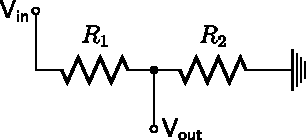
\includegraphics[width=0.35\textwidth]{graphics/03_temperature/resistive_divider.pdf}
    \caption{A resistive voltage divider. After \href{https://en.wikipedia.org/wiki/Voltage_divider\#/media/File:Resistive_divider2.svg}{Krishnavedala via Wikipedia}, \href{https://creativecommons.org/publicdomain/zero/1.0/deed.en}{CC0}.}
    \label{fig:temperature:voltage_divider}
\end{figure}
Figure~\ref{fig:temperature:voltage_divider} shows a schematic of a voltage divider built of two resistors with values $R_1$ and $R_2$. The current flows from $V_\mathrm{in}$ to ground. We can calculate the voltage measured between $V_\mathrm{out}$ and ground as following.
\begin{align}
    R_\mathrm{tot} &= R_1 + R_2 \label{eqn:temperature:voltage_divider:rtot} \\
    I_\mathrm{tot} &= \frac{V_\mathrm{in}}{R_\mathrm{tot}} \label{eqn:temperature:voltage_divider:itot} \\
    V_\mathrm{out} &= R_2 I_\mathrm{tot} \label{eqn:temperature:voltage_divider:vout_first_step}\\
    V_\mathrm{out} &= V_\mathrm{in} \frac{R_2}{R_1 + R_2} \label{eqn:temperature:voltage_divider:final}
\end{align} 
In equation~\eqref{eqn:temperature:voltage_divider:rtot} we first calculate the total resistance of the setup. Plugging this result into equation~\eqref{eqn:uri}, we can calculate the total current flowing, equation~\eqref{eqn:temperature:voltage_divider:itot}. Since $V_\mathrm{out}$ is measured over $R_2$, we can simply calculate the voltage over this element as in equation~\eqref{eqn:temperature:voltage_divider:vout_first_step}, which when simplified results in equation~\eqref{eqn:temperature:voltage_divider:final}. More details, as well as more general voltage divider setups, can be found on \href{https://en.wikipedia.org/wiki/Voltage_divider}{Wikipedia}.

\subsection{Using a thermistor with an \ac{adc}}

In order to determine the resistance of a thermistor and thus to determine the temperature, we can use above described voltage divider setup. For example, we could use a reference resistance $R_\mathrm{ref}$ instead of $R_1$ in Figure~\ref{fig:temperature:voltage_divider} and replace $R_2$ with the thermistor that has a resistance $R_\mathrm{therm}$. Connecting $V_\mathrm{out}$ to an \ac{adc}, we can then determine the thermistor resistance by solving equation~\ref{eqn:temperature:voltage_divider:final} for $R_2 \equiv R_\mathrm{therm}$. We can thus write
\begin{equation}
    R_\mathrm{therm} = \frac{R_\mathrm{ref}}{\frac{V_\mathrm{in}}{V_\mathrm{out}} - 1}.
    \label{eqn:temperature:rtherm_voltage_divider}
\end{equation}
For an \ac{adc} with $n$\,bit resolution, we furthermore know that the measured value $x$ relates to the voltage as
\begin{equation}
    V_\mathrm{out} = \frac{x \cdot V_\mathrm{ref,ADC}}{2^{n} - 1},  \label{eqn:temperature:adc_conversion}
\end{equation}
where $V_\mathrm{ref,ADC}$ is the reference voltage of the \ac{adc}. 
Plugging equation~\eqref{eqn:temperature:adc_conversion} into~\eqref{eqn:temperature:rtherm_voltage_divider} results in
\begin{equation}
    R_\mathrm{therm} = \frac{R_\mathrm{ref}}{\frac{(2^{n} - 1) \cdot V_\mathrm{in}}{x\cdot V_\mathrm{ref,ADC}} - 1}.
\end{equation}
If the reference voltage of the \ac{adc} and the reference voltage of our voltage divider setup are the same, we can further simplify the equation to
\begin{equation}
    R_\mathrm{therm} = \frac{R_\mathrm{ref}}{\frac{2^{n} - 1}{x} - 1}.
\end{equation}

\subsection{Determining the temperature}\label{sec:temperature:thermistor:determining_temperature}

Knowing the resistance $R_\mathrm{therm}$ of the resistor, we can determine the temperature by looking up the correct value in a lookup table, see the \ac{csv} file on \href{https://github.com/galactic-forensics/workshop_arduino_electronics/blob/main/figures/03_temperature/thermistor_lookup_table_adafruit_372.csv}{GitHub}.

The temperature can also be calculated using the \href{https://en.wikipedia.org/wiki/Steinhart%E2%80%93Hart_equation}{Steinhard-Hall} equation, which is a model for the resistance of a semiconductor at different temperatures. This model states that the temperature $T$ and resistance $R_\mathrm{therm}$ depend on each other as
\begin{equation}
    \frac{1}{T} = a + b\ln{R} + c \left(\ln{R}\right)^{3}. \label{eqn:temperature:steinhard_hall}
\end{equation}
Here, $a$, $b$, and $c$ are constants. Doing a curve fit of this equation to the lookup table for the thermistor, we can determine the constants as $a=2.78522\times10^{-3}\,\mathrm{K}^{-1}$, $b=2.41846\times10^{-4}\,\ln({\mathrm{k}\Omega})^{-1}$, and $c=8.31227\times10^{-7}\,\ln({\mathrm{k}\Omega})^{-3}$. 

A simplified version of above equation, the so-called B-parameter equation (see \href{https://en.wikipedia.org/wiki/Thermistor}{Wikipedia}) assumes that the constants are $a=1/T_0 - (1/B)\ln{R_0}$, $b=1/B$, and $c=0$. We can therefore rewrite equation~\eqref{eqn:temperature:steinhard_hall} as
\begin{equation}
    \frac{1}{T} = \frac{1}{T_0} + \frac{1}{B} \ln\left( \frac{R}{R_0} \right). \label{eqn:temperature:thermistor}
\end{equation}
Here, $T_0 = 298.15\,$K is room temperature and $R_0 = 10\,\mathrm{k}\Omega$ the resistance at $T_0$. The parameter $B$ for \href{https://www.adafruit.com/product/372}{our thermistor} is $B=3950\,$K.

\begin{figure}[tbh]
    \centering
    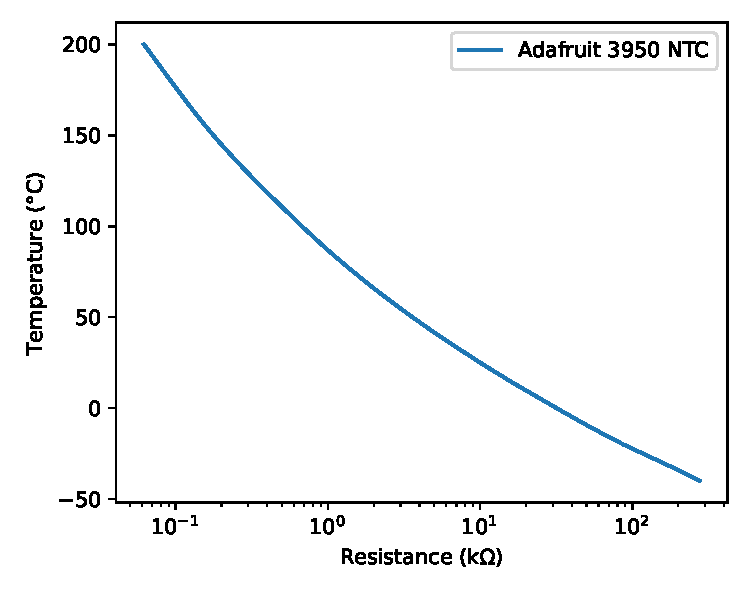
\includegraphics[width=0.625\textwidth]{graphics/03_temperature/thermistor.pdf}
    \caption{Temperature as a function of resistance for \href{https://www.adafruit.com/product/372}{Adafruit 3950 NTC} thermistor}
    \label{fig:temperature:thermistor}
\end{figure}
Figure~\ref{fig:temperature:thermistor} shows the temperature determined using the lookup table in comparison with fitting the Steinhard-Hall equation~\eqref{eqn:temperature:steinhard_hall} and the B-parameter equation~\eqref{eqn:temperature:thermistor} results. While the B-parameter equation gets close to the real values, it still has a significant offset. The Steinhard-Hall fit to the lookup table on the other hand seems to be a fairly good match.

\qbox{How will you determine the temperature? The lookup table has the most precision, however, what would you do with a resistance that is in between two values in the table? Our setup will have an actual temperature range between around 25\celsius and -20\celsius. How well do the methods compare in this range?}

\qbox{The Arduino Micro has a 10\,bit ADC on board. Assuming a reference resistor $R_\mathrm{ref} = 10\,\mathrm{k}\Omega$, calculate the smallest temperature difference that you would be able to determine with this ADC in the above defined temperature range. }

\section{Reading the temperature with the Arduino}

We will now use the thermistor in order to measure the room temperature. With above introduction, you should be ready to build the setup by yourself. However, there are also detailed instructions available on \href{https://learn.adafruit.com/thermistor/using-a-thermistor}{Adafruit's website} on how to set this up correctly. Note however the uncertainties in the different approaches for determining the temperature shown in Figure~\ref{fig:temperature:thermistor}.

\exerbox{Connect the thermistor using the provided reference resistor to your Arduino and measure the voltage on any of the analog input pins (ADC[0] through ADC[7] in Figure~\ref{app:pinout}). If you connect your input to \lstinline{sensorPin = A0;}, you can read the ADC value by calling \lstinline{sensorValue = analogRead(sensorPin);}. Read the resistance value out using the serial monitor. If you have trouble reading from the ADC, check out the Arduino example under ``Analog'', ``AnalogInput''. \textit{Note:} Make sure that the reference voltage of the ADC is the same voltage as the one you are using for $V_\mathrm{in}$.}

\morebox{\lstinline{int sensorPin = A0;}}{In above exercise, the \ac{adc} pin was initialized as an integer with the value \lstinline{A0}. Why does this not throw an error?}

\exerbox{In Section~\ref{sec:temperature:thermistor:determining_temperature} we have discussed various approaches of determining the temperature. Implement your solution from above's question in order to calculate the temperature and print it out using the serial monitor. How precise are your readings? Does your room temperature measurement make sense?}

\exerbox{Instead of printing the temperature via the serial monitor, display the temperature on the four-digit, seven-segment display that you have controlled in Chapter~\ref{chap:display}. Be concious about the environment and recycle -- even your code!}

\begin{figure}[tb]
    \centering
    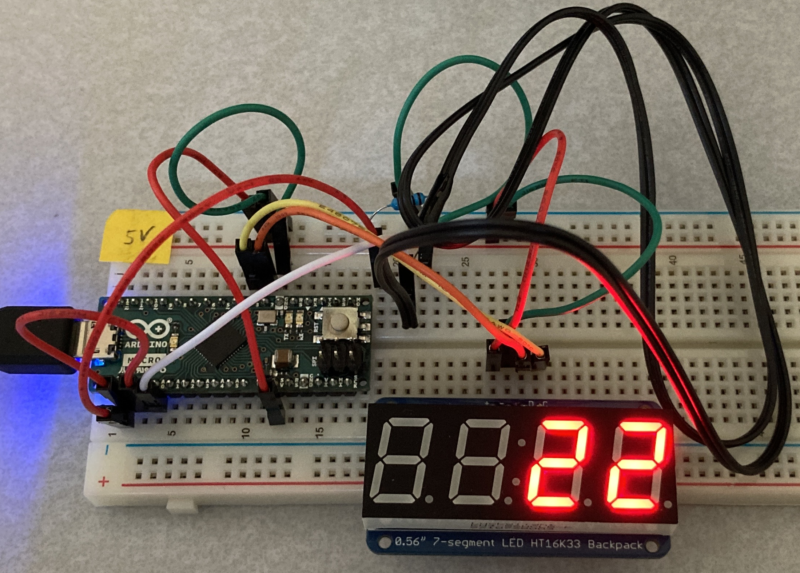
\includegraphics[width=0.625\textwidth]{graphics/03_temperature/final_setup.png}
    \caption{Temperature reading via thermistor and shown using the the four-digit, seven-segment display.}
    \label{fig:temperature:final_setup}
\end{figure}
Figure~\ref{fig:temperature:final_setup} shows the final setup after the last exercise. Note that your setup might of course look slightly different.

Your temperature readings might be varying a lot from measurement to measurement. The reason for this is electronic noise. There are two ways of reducing the effects of such noise: (1) For your result use the average of several measurements. (2) The 5\,V line of the Arduino is fairly unfiltered and depends on the power supply you are using. The 3.3\,V Arduino line (see Figure~\ref{app:pinout}) on the other hand is fairly stable, and it would therefore be advantageous to use this line for ADC measurements. To do so, switch your $V_\mathrm{in}$ to use the 3.3\,V line. You can provide this line to the ADC as a reference voltage. To do so, also connect the \lstinline{AREF} pin to the same 3.3\,V line.

\exerbox{Using above methods of averaging and using the 3.3\,V as your measurement and reference voltage, determine if your temperature measurements improve.}

Finally, as Physicists we know that an ice-water mixture at standard pressure and temperature (we are close to the ocean, so let's assume that's given) is by definition at 0\celsius. The thermistor that you have is waterproof, and you can therefore submerge in such a ``calibration solution''.

\exerbox{Determine the temperature of an ice-water mixture using your code. How precise is your determination of the temperature? If you are off by several degrees, there might be an error in your temperature measurement capability and your code might need correction.}